\chapter{Design and Implementation\label{chapter:design}}

\section{Shared specification: the fairness baseline}
\label{sec:fairness}
One specification, frozen before any code was written and naming no language, fixes the public
API, the UE state machine, the data structures and their algorithms (a sharded hash map keyed by
UE identifier, for instance), locking and sharding granularity, and the concurrency model. Both
implementations follow it, so this compares two languages, not two designs or two skill levels.
The specification is a deliverable in its own right and the main control against implementation
bias.

\section{Conceptual model and concurrency design}\label{sec:concurrency}
Two implementations are built against it: modern C++ (C++23, the Standard Template Library (STL),
RAII, standard threading) and Rust (stable toolchain, ownership-based memory model, safe
concurrency). Both use one concurrency model, \emph{shared-nothing, thread-per-shard}, which is
how real RAN layer 3 divides UE state, and neither mixes async with thread-based models,
deliberately.

Shards partition the UE-identifier space, $N_{\text{shards}}$ of them, one worker thread each,
eight by default. The reported campaign runs seven workers and seven producers, well inside
Section~\ref{sec:testbed}'s $\MainPinnedCount$ pinned cores and inherited from the earlier host,
where fourteen threads met fourteen pinned cores exactly. Section~\ref{sec:controls} requires the
count to match across languages, as it does in every campaign, not across machines: the second
bare-metal campaign raises it to \BmShards{} deliberately, to test whether the findings depend on
the choice (Section~\ref{sec:hostcompare}). Only the owning worker reads or changes its shard's
contexts, so nothing mutable is shared, context data needs no locks, and the load generators never
touch that state. They submit request messages to a shard's bounded multi-producer,
single-consumer (MPSC) queue, then wait on a single-use completion handle the worker writes the
result into. Submission on a full queue blocks until space frees, producing realistic queueing
latency under overload and making tail latency observable at all, where dropping requests would
hide it. Same-shard requests run strictly first in, first out (FIFO).

Under test, then, and what gives the safe-concurrency comparison something to measure, are the
queue, the completion handoff and each request's ownership transfer, not lock contention. One
piece of shared mutable state is allowed: an atomic counter stamping a per-context activity
sequence number, write-only bookkeeping no control flow branches on. Latency spans the whole
path, from intended send time to completion, taking in queueing delay under load and the same
cross-thread round-trip on both sides, a figure Section~\ref{sec:budget} splits between language
and operating system. Figure~\ref{fig:arch} gives the data flow, Figure~\ref{fig:reqlifecycle}
one operation's path through it.

\begin{figure}[ht]
\centering
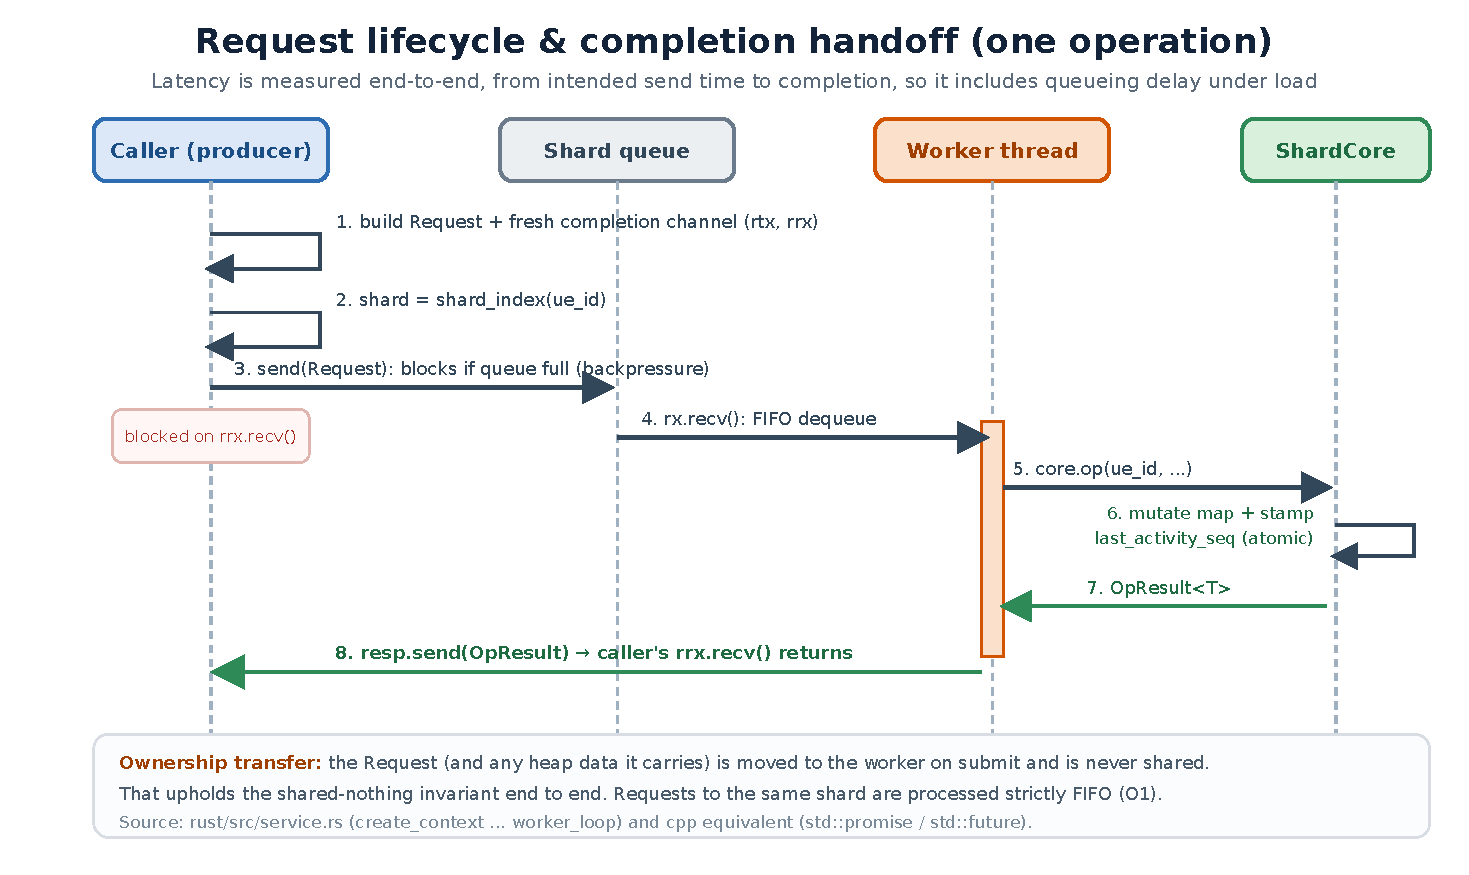
\includegraphics[width=0.78\linewidth]{diagrams/pdf/04_request_lifecycle_sequence.pdf}
\caption[The end-to-end path of a single operation]{The end-to-end path of a single operation and the completion handoff, routed by
\texttt{shard\_index(ue\_id)} and executed against the shard's exclusively owned store. Ownership
of the request transfers to the worker on submit and is never shared. Latency is measured across
the whole path.\label{fig:reqlifecycle}}
\end{figure}

\begin{figure}[ht]
\centering
\begin{tikzpicture}[
    font=\small,
    prod/.style={draw, rounded corners, minimum width=2.0cm, minimum height=0.66cm, fill=blue!8},
    queue/.style={draw, minimum width=2.5cm, minimum height=0.66cm, fill=gray!12},
    worker/.style={draw, rounded corners, minimum width=2.1cm, minimum height=0.66cm, fill=red!8},
    store/.style={draw, cylinder, shape border rotate=90, aspect=0.25, minimum width=1.5cm, minimum height=0.85cm, fill=green!8},
    lane/.style={draw, dotted, rounded corners, inner sep=7pt},
    >={Stealth[length=2.4mm]}
  ]
  % producers, grouped in one box to avoid a tangle of crossing arrows
  \node[prod] (p1) at (0,1.3)  {Producer 1};
  \node[prod] (p2) at (0,0.0)  {Producer 2};
  \node[prod] (p3) at (0,-1.3) {Producer $m$};
  \begin{scope}[on background layer]
    \node[draw, dashed, rounded corners, fill=blue!3, fit=(p1)(p2)(p3), inner sep=6pt] (pg) {};
  \end{scope}
  \node[font=\scriptsize] at (0,-2.15) {load generators};

  % two representative shard lanes; spacing leaves room for the inline edge labels
  \node[queue] (q1) at (5.2,1.3)   {MPSC queue};
  \node[worker](w1) at (8.9,1.3)   {Worker 1};
  \node[store] (s1) at (12.0,1.3)  {Shard 1};
  \node[queue] (qn) at (5.2,-1.3)  {MPSC queue};
  \node[worker](wn) at (8.9,-1.3)  {Worker $N$};
  \node[store] (sn) at (12.0,-1.3) {Shard $N$};
  \begin{scope}[on background layer]
    \node[lane, fit=(q1)(s1)] (lane1) {};
    \node[lane, fit=(qn)(sn)] (lanen) {};
  \end{scope}
  \node[font=\scriptsize] at (8.35,2.35) {shard-owning threads: no shared mutable state, no locks};

  % submit: producer group -> each shard queue, routed by hash
  \node[font=\scriptsize, align=center, fill=white, inner sep=2pt] at (2.85,0) {route by\\ hash(\texttt{ue\_id})};
  \draw[->] (pg.east) -- (q1.west) node[midway, above, sloped, font=\scriptsize]{submit};
  \draw[->] (pg.east) -- (qn.west) node[midway, below, sloped, font=\scriptsize]{submit};

  % within-lane flow
  \draw[->]  (q1) -- node[above, font=\scriptsize]{FIFO} (w1);
  \draw[->]  (qn) -- node[above, font=\scriptsize]{FIFO} (wn);
  \draw[<->] (w1) -- node[above, font=\scriptsize]{owns} (s1);
  \draw[<->] (wn) -- node[above, font=\scriptsize]{owns} (sn);

  % one-shot completion: clean orthogonal return path below everything
  \draw[->, dashed, rounded corners=4pt]
      (wn.south) -- ++(0,-0.75) -- (1.4,-2.9) -- ($(pg.south east)+(-0.4,0)$);
  \node[font=\scriptsize] at (5.9,-3.05) {one-shot completion (result $\rightarrow$ waiting producer)};
\end{tikzpicture}
\caption[Shared-nothing, thread-per-shard architecture]{Shared-nothing, thread-per-shard architecture. Queues are bounded and blocking and their
shard is selected by a pinned hash of the \texttt{ue\_id}. Exactly one worker thread reads and
writes each shard, so context state needs no locks, and blocking on a full queue is what makes
overload observable as tail latency.\label{fig:arch}}
\end{figure}

\section{Architectural choices and technology stack}
C++ builds with CMake and Ninja on the standard library and \texttt{std::thread}, Rust with Cargo
on the stable toolchain. Both link the same memory allocator, keeping the comparison about two
languages and not two allocators: C++ the system \texttt{jemalloc}, Rust a \texttt{jemalloc}
global allocator from \texttt{tikv-jemallocator}. Each side also keeps a system-allocator build
as a control. Latency passes through the same HDR histogram
algorithm~\cite{tene_hdrhistogram} on both sides, identically configured (range
$[1\,\text{ns}, 3.6\,\text{s}]$, three significant figures), from Rust's standard
\texttt{hdrhistogram} crate and a C++ header-only port of the same bucketing algorithm, checked
against a known distribution. Optimisation is matched as closely as the toolchains allow, the
Rust release profile pinned to \texttt{opt-level~=~2} against C++ \texttt{-O2}.

\section{Implementation details}\label{sec:impldetails}
\label{sec:impl}
Both cores follow the specification field for field and are small enough to read end to end.
The C++ core is $\CppRawLines$ lines across eight headers and two translation units, the Rust core
$\RustRawLines$ across eight modules, or $\CppNloc$ and $\RustNloc$ without blank lines and
comments. Both counts describe the build the campaign measures: a flag switches on the two
attribution probes of Section~\ref{sec:idioms}, and the conditional blocks selecting them are
left out, since counting them would describe neither the compared build nor the probe.

Rust is therefore the larger core, by $\RawRise\%$ in raw lines and $\NlocRise\%$ in code lines.
Line count is one of the software-quality proxies this study set out to collect, and the
difference is not stray verbosity but the net of several forced idioms pulling in opposite
directions, which Section~\ref{sec:idioms} takes apart file by file. Three carry a measured
consequence: a record layout differing by $\UeCtxGapBytes$~bytes per context, the request
representation, in both size and type safety, and the bounded queue. The rest is naming or
mechanism, and though several of those cost source lines, which Table~\ref{tab:loc} accounts for,
none changes what the two cores do. Appendix~\ref{appendix:impl} walks the three constructions
field by field.

\subsection{The UE context and the state machine}\label{sec:uecontext}
Each UE context stores the fields Figure~\ref{fig:datamodel} sets out: identifier, a four-value
lifecycle state, a dummy security context, a growable bearer list, and the cell, transaction and
counter fields. The bearer list is a \texttt{std::vector} / \texttt{Vec} so that RQ3 observes
realistic per-context allocation, and reads return an immutable snapshot copied out of the worker.
Identical declarations do not produce identical objects. A \texttt{UeContext} takes
$\CppUeCtxBytes$~bytes in C++ and $\RustUeCtxBytes$~bytes in Rust, because C++ keeps declaration
order where Rust packs the scalars, and the specification does not erase that gap:
\texttt{\#[repr(C)]} would penalise Rust for a C++ padding rule, and reordering the C++
declarations is an optimisation neither side is asked for. At $\SweepUes$ active UEs the gap is
roughly $\UeCtxGapTotalKB$~kB, two orders of magnitude below Chapter~\ref{chapter:eval}'s
resident-set difference.

\begin{figure}[ht]
\centering
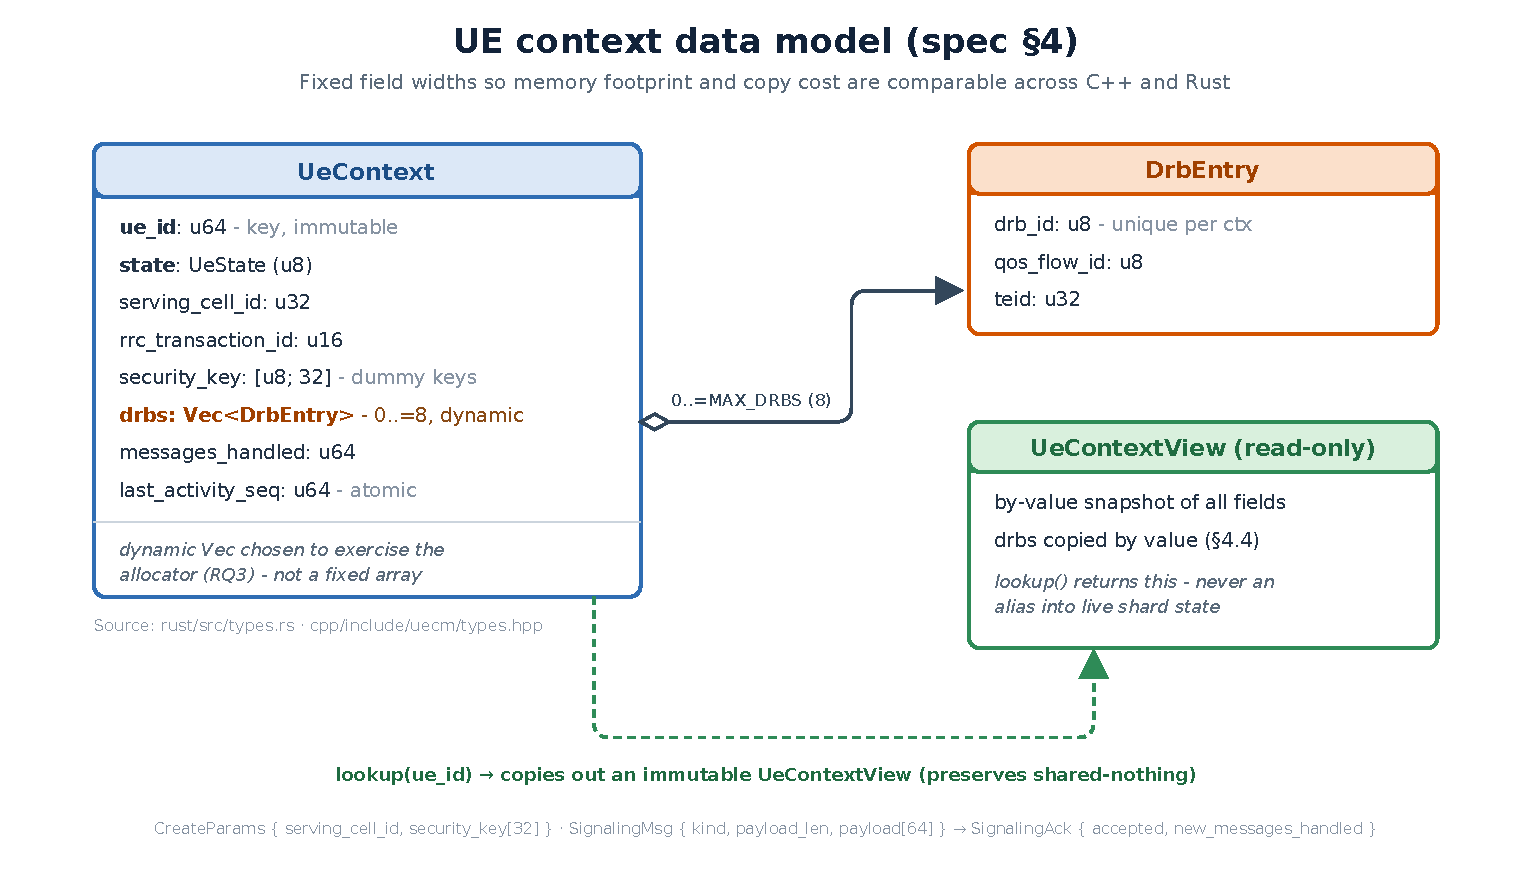
\includegraphics[width=0.72\linewidth]{diagrams/pdf/05_data_model.pdf}
\caption[The shared UE-context data model]{The UE-context data model shared by both implementations. Field widths are fixed so that
memory footprint and copy cost are comparable across languages, and the data-radio-bearer list is
dynamic on purpose, to exercise the allocator for RQ3. \texttt{lookup} returns an immutable
\texttt{UeContextView} copied out by value, not an alias into live shard state, preserving the
shared-nothing guarantee.\label{fig:datamodel}}
\end{figure}

\subsection{Sharding, the store, and the bounded queue}
Both sides pin hashing so that neither standard library's hasher becomes a language advantage.
Shard assignment puts the \texttt{ue\_id} through the SplitMix64 finalizer and reduces modulo the
shard count, spreading sequential identifiers, and inside the shard both maps are keyed through a
pinned FNV-1a 64-bit hash, with a test checking the Rust \texttt{BuildHasher} bit-identical to the
reference. Capacity is reserved at start-up. Table~\ref{tab:params} lists the rest.

The bounded blocking queue is where the libraries part company. Rust supplies
\texttt{sync\_channel(capacity)} outright. C++23 has no such primitive, so the same semantics are
assembled by hand from a \texttt{mutex}, two \texttt{condition\_variable}s and a
\texttt{std::queue}, in a class of $\CppBoundedQueueLines$ lines. Those lines are where a
concurrency defect could enter, and their correctness argument rests with the author, not the
compiler. Appendix~\ref{appendix:impl} records the construction.

\subsection{Requests, responses, and the service lifecycle}\label{sec:tagged}
\label{sec:request}
Rust models a request as an \texttt{enum} sized by its largest variant
($\RustRequestBytes$~bytes). C++ uses a tagged struct carrying every argument field
($\CppRequestBytes$~bytes) plus a \texttt{std::variant} of four result types the caller unwraps
with \texttt{std::get}, so full occupancy of the default queues is roughly
$\CppQueueResidentMB$~MB against $\RustQueueResidentMB$~MB. The invariant that the stored
alternative matches the \texttt{OpKind} is upheld by reading two files. Rust settles it by
construction.

Shutdown pushes an in-band \texttt{Stop} sentinel onto each shard's queue, and FIFO order
completes every request ahead of it. Both languages tie start and stop to object destruction.
The window between \texttt{start()} and \texttt{shutdown()} is a precondition the specification
wrote and neither implementation first checked. C++ then faults and Rust panics. The episode is
reported with the safety results in Section~\ref{sec:safetyresults}.
A request is moved into the queue, not copied, so producer and worker never both hold a usable
reference. Appendix~\ref{appendix:impl} gives the request layout and the lifecycle gap as found.

\subsection{Forced idioms, and what the two cores cost}
\label{sec:idioms}
Where the two languages must diverge to meet the same requirement, the deviation goes into the
specification's forced-idiom log, to be weighed rather than silently absorbed into the results.
Table~\ref{tab:idioms} collects it in full, and the two entries with measurable consequences are
quantified above.

\begin{table}[H]
\centering
\small
\caption[The forced-idiom log]{The forced-idiom log: every point at which the two implementations diverge in order
to satisfy the same specification requirement, with the measured consequence where there is
one.\label{tab:idioms}}
\begin{tabular}{@{}R{0.20\linewidth} R{0.36\linewidth} R{0.36\linewidth}@{}}
\hline\hline
Concern & C++ & Rust \\
\hline
Result type & \texttt{std::expected<T, OpError>} & \texttt{Result<T, OpError>} \\
Request & tagged struct: discriminant plus every argument field ($\CppRequestBytes$\,B) & \texttt{enum}, one variant per operation, carrying only its own arguments ($\RustRequestBytes$\,B) \\
Response & \texttt{std::variant} of four result types, unwrapped by the caller with \texttt{std::get} & none needed: each variant carries a sender of its own result type \\
Bounded queue & hand-written \texttt{mutex} plus two \texttt{condition\_variable}s ($\CppBoundedQueueLines$ lines) & \texttt{sync\_channel(capacity)} \\
Completion & \texttt{std::promise} / \texttt{std::future} & a fresh \texttt{mpsc::channel()} per request \\
Per-shard map & \texttt{std::unordered\_map} with an \texttt{FnvHash} functor & \texttt{HashMap} with an \texttt{FnvBuildHasher} \\
Activity counter & \texttt{std::atomic<uint64\_t>} held by reference & \texttt{Arc<AtomicU64>} cloned into each worker \\
Teardown & destructor calls \texttt{shutdown()} & \texttt{Drop} calls \texttt{shutdown()} \\
Optimisation level & \texttt{-O2} & \texttt{opt-level = 2} \\
\hline
\end{tabular}
\end{table}

Table~\ref{tab:loc} breaks the $\LocGap$-line gap down by concern. Rust is shorter in exactly one
place, the bounded queue, needing no code against $\CppBoundedQueueLines$ lines of C++, and longer
almost everywhere else, mostly in three entries: the service module, whose per-variant typed
sender admits no shared helper, the hasher trait apparatus, and the module tree C++ gets from its
header structure. None of it shows up in the performance figures. Rust spends lines on trait
machinery and call-site repetition, winning much of that back wherever its standard library
supplies a primitive C++'s does not.

Counting lines treats boilerplate and branching alike, answering only half the question, so
Table~\ref{tab:complexity} adds cyclomatic complexity, measured by \texttt{lizard}~\cite{lizard}
over both cores. One tool on both languages applies one definition of a decision point, where
each language's own tooling would count somewhat different things, and that is what makes the
figures comparable. The two measures point in opposite directions. Rust is $\NlocRise\%$ longer
than C++ by code lines, but its total cyclomatic complexity is $\CcnTotalDrop\%$ \emph{lower},
$\RustCcnTotal$ against $\CppCcnTotal$, over slightly more functions ($\RustFuncs$ against
$\CppFuncs$). Both cores are undemanding by the usual thresholds, with a median per-function
complexity of one, so a few functions at the top carry the aggregate.

That top is where the difference sits. The C++ core's most complex function is $\CppCcnMaxFn$ at
$\CppCcnMax$, more than twice its Rust counterpart's $\RustCcnMax$. It switches on the
\texttt{OpKind} discriminant and stores the matching alternative into the response
\texttt{variant}, so Section~\ref{sec:tagged}'s tagged-struct design gathers the whole dispatch
into one branch-heavy function, where Rust's per-variant typed sender removes the return-path
dispatch and leaves its worker nothing comparable to unwrap. Rust's extra lines buy back branching
where branching is hardest to review, and the \texttt{std::bad\_variant\_access} invariant upheld
by reading two files lives inside exactly the function this measurement flags.

\begin{table}[H]
\centering
\small
\caption[Size and cyclomatic-complexity proxies for the two cores]{Size and cyclomatic-complexity proxies for the two cores, measured with
\texttt{lizard}~\cite{lizard} applied identically to both languages. Benchmark drivers, tests,
conformance runners, the FFI seam, and the probe-conditional blocks of
Section~\ref{sec:idioms} are excluded, so only the compared code the parity contract constrains
is counted. Complexity is one plus the number of decision points in a function. The line count
is non-commenting lines of code (NLOC) as \texttt{lizard} defines it, discounting brace-only and
preprocessor lines, and quoted at the head of
Section~\ref{sec:impldetails}.\label{tab:complexity}}
\begin{tabular}{@{}l r r@{}}
\hline\hline
Measure & C++ & Rust \\
\hline
Files & 10 & 8 \\
Functions & 37 & 42 \\
Lines of code (blank and comment lines excluded) & 517 & 621 \\
Total branching complexity & 95 & 83 \\
Mean complexity per function & 2.6 & 2.0 \\
Median complexity per function & 1 & 1 \\
Most complex function & 13 (\texttt{worker\_loop}) & 6 (\texttt{add\_drb})
\\
\hline
\end{tabular}
\end{table}

\begin{table}[H]
\centering
\small
\caption[Where the line-count difference between the cores comes from]{Where the $\LocGap$-line difference between the two cores comes from, by concern (raw
lines, including comments. C++ figures merge header and translation unit. Probe-conditional
blocks excluded as in Section~\ref{sec:impldetails}). Rust is shorter
only where its standard library supplies a primitive C++ lacks.\label{tab:loc}}
\begin{tabular}{@{}R{0.38\linewidth} r r r@{}}
\hline\hline
Concern & C++ & Rust & $\Delta$ \\
\hline
Service (queues, workers, API) & $234$ & $291$ & $+57$ \\
Hashing (functor vs.\ trait pair) & $37$ & $70$ & $+33$ \\
Module tree and re-exports & $0$ & $26$ & $+26$ \\
Message types & $48$ & $67$ & $+19$ \\
Data model & $73$ & $85$ & $+12$ \\
Configuration & $18$ & $29$ & $+11$ \\
Shard core (state machine) & $182$ & $188$ & $+6$ \\
Error model & $32$ & $26$ & $-6$ \\
Bounded queue & $51$ & $0$ & $-51$
\\
\hline
Total                             & $\CppRawLines$ & $\RustRawLines$ & $+\LocGap$ \\
\hline
\end{tabular}
\end{table}

Two properties of the Rust core are not costs but what the costs bought. The library contains
\emph{no} \texttt{unsafe} code and resolves no third-party crate, depending on the standard
library alone, so nothing outside it is compiled into the artefact this study measures. Both are
checked mechanically over the crate rather than asserted, and Section~\ref{sec:migrationresults}
reports the counts. Safe Rust therefore guarantees this core data-race freedom at compile time,
through the \texttt{Send} and \texttt{Sync} traits: a single worker owns each shard store and never
shares it, the request type is moved across the thread boundary, and the one genuinely shared
piece of state, the activity counter, is an atomic. None of it needs a runtime sanitiser to
establish or test coverage to hold. The C++ implementation does no manual memory management beyond
STL containers and no explicit locking outside the queue class, and was checked data-race free
under ThreadSanitizer.

The two statements are not evidence of the same kind, and that difference is the thesis's central
safety claim in miniature. The Rust property is a theorem about the program, discharged by the
compiler on every ordinary build, covering every execution. The C++ property is an observation
about the executions one instrumented binary happened to take, to be re-established after any
change, on a build most projects do not run by default. Quantifying how far apart the two kinds of
assurance are is the purpose of Chapter~\ref{chapter:eval}'s fault-injection study.

\section{Public API and operation semantics}
Both implementations expose the same small, lifecycle-oriented API, so the surface a caller sees
is identical apart from naming conventions. A service is created with a fixed shard count and a
per-shard queue bound. Callers then invoke context operations, each identified by the target
\texttt{ue\_id}: create, setup, handle-signalling, add-bearer, reconfigure
begin/complete/abort, release, and state lookup. Every operation is \emph{total} and
\emph{typed}, returning either a success value or a typed \texttt{OpError} from a closed
five-value enumeration (\texttt{NotFound}, \texttt{AlreadyExists}, \texttt{InvalidState},
\texttt{CapacityExceeded} and \texttt{InvalidArgument}). An operation illegal for the context's
current state (Figure~\ref{fig:fsm}) returns the matching error, leaves the context untouched,
and signals no failure out of band.

That matters for fairness as much as for correctness. Neither implementation uses
exceptions or error codes as a hidden control-flow channel, so the failure path is visible and
identical on both sides, and the same conformance vectors (Section~\ref{sec:parity}) can assert
op-for-op agreement on the returned value and the resulting state. Two points the drawn state
machine hides still need stating. \texttt{Released} is never stored, since
\texttt{release\_context} erases the entry, so a second release returns \texttt{NotFound} and not
\texttt{InvalidState}. And \texttt{abort\_reconfigure} restores the \emph{state} to
\texttt{Connected} without restoring the serving cell \texttt{begin\_reconfigure} overwrote, the
model keeping none to roll back to. The parity suite holds both languages to both commitments.

\section{Parity verification}
\label{sec:parity}
The comparison rests on the two versions being functionally identical, so parity is tested, not
assumed. A language-neutral conformance suite writes test vectors as operation sequences with
their expected results and post-state summary, a runner in each language executes them and emits a
transcript in one fixed format, and the two transcripts are diffed for op-for-op agreement. The
seeded suite covers the full error model, the reconfiguration begin/complete/abort paths,
data-radio-bearer fill and overflow, and shard-assignment determinism. Both implementations
currently pass and agree. The benchmark workloads add a second parity signal, independent of the
first: for a given seed and active-UE population, the mixed workload's per-operation-kind counts
are checked identical across languages, confirming that both are driven along exactly the same
code paths.

Two things bound what that establishes, and both are answered rather than conceded. A cross-diff
of two implementations cannot tell ``both correct'' apart from ``both wrong in the same way''. A
third implementation of the same written specification therefore acts as an independent oracle:
written in Python, sharing no code with either language, it must reproduce all $\ConfHandOps$
hand-derived expectations before it may generate any of its own. It then generates randomised
operation sequences, and a campaign of roughly $\ConfGenOps$ generated operations produced no
divergence at all. The generator is seeded and deterministic, so any future divergence is a
permanently reproducible regression.

Three further checks bound the suite from other directions. The specification's transition matrix
is walked exhaustively: every operation applied to a context in every state it can occupy,
asserting the exact error, the resulting state on success, and the absence of any field change on
failure. The C++ implementation then runs under AddressSanitizer, ThreadSanitizer and
UndefinedBehaviorSanitizer across that whole suite and reports nothing, and Miri over the Rust
state-machine suite likewise reports no undefined behaviour. Line coverage of the C++ library is
$\CppLineCov\%$ and of the Rust library $\RustLineCov\%$, with both cores' operation processors
and service facades fully covered ($\RustRegionCov\%$ on the finer-grained regions
\texttt{llvm-cov} counts).
